% ============================================================================
%  Project Specification and Preliminary Report — 中文对照版（阅读用，非提交版）
%  Build:  xelatex -> bibtex -> xelatex -> xelatex
% ============================================================================
\documentclass[10pt,a4paper]{article}

\usepackage[UTF8]{ctex}
\usepackage{fontspec}
\setmainfont{Times New Roman}
\setsansfont{Arial}
\setmonofont{Consolas}

\usepackage[a4paper,top=1.8cm,bottom=1.7cm,left=2.1cm,right=2.1cm]{geometry}
\usepackage{graphicx}
\usepackage{float}
\usepackage{booktabs}
\usepackage{array}
\usepackage{amsmath}
\usepackage{xcolor}
\usepackage{enumitem}
\usepackage{caption}
\usepackage{fancyhdr}
\usepackage[hidelinks]{hyperref}
\usepackage{parskip}
\setlength{\parskip}{3pt plus 1pt}
\setlength{\parindent}{0pt}
\usepackage{tikz}
\usetikzlibrary{arrows,positioning,fit,backgrounds}
\usepackage[htt]{hyphenat}
\setlength{\emergencystretch}{2.5em}

\captionsetup{font=small,labelfont=bf,skip=4pt}
\setlist[itemize]{leftmargin=1.3em,topsep=2pt,itemsep=1pt}
\setlist[enumerate]{leftmargin=1.6em,topsep=2pt,itemsep=1pt}

\pagestyle{fancy}
\fancyhf{}
\fancyhead[L]{\small\itshape Project Specification and Preliminary Report · 中文对照}
\fancyhead[R]{\small\itshape Xu Yuxuan, 2959485}
\fancyfoot[C]{\small\thepage}
\renewcommand{\headrulewidth}{0.4pt}

\newcommand{\code}[1]{\texttt{\small #1}}

% 中文译文块：灰色小一号，行首一个「中」标记，与英文正文区分开
\newenvironment{zh}{%
  \par\vspace{1pt}%
  \begingroup
  \color{black!72}\small
  \setlength{\parskip}{0pt}%
  \noindent\textsf{\footnotesize 中}\hspace{3pt}\ignorespaces
}{%
  \par\endgroup\vspace{4pt}%
}

\begin{document}

% ---------------------------------------------------------------------------
%  Cover block
% ---------------------------------------------------------------------------
\begin{center}
  {\large\bfseries Design and Development of an AI-Enabled Smart Electric Vehicle\\
   Charging and Energy Management Platform}\\[4pt]
  {\normalsize Project Specification and Preliminary Report}\\[2pt]
  {\small Sub-project 1: EV Charging Data Analysis and Demand Forecasting}\\[2pt]
  {\small University of Glasgow \,|\, Glasgow College UESTC, Hainan \,|\, UESTCHN4008P}\\[4pt]
  {\small\color{black!65} 中文对照版 · 仅供本人阅读与组会讲解；提交请使用英文版（页数上限 8 页）}
\end{center}

\vspace{-2pt}
{\small
\renewcommand{\arraystretch}{1.15}
\begin{tabular}{@{}p{3.5cm}p{6.6cm}p{2.9cm}p{1.9cm}@{}}
\toprule
Student name & Xu Yuxuan & Matriculation & 2959485 \\
UESTC student number & 2959485 & Academic year & 2026--27 \\
First supervisor & Dr Amer Ghias & Placement company & --- \\
Degree programme & Electronics and Information Engineering & & \\
Working title & AI-enabled smart EV charging and energy management platform & & \\
\bottomrule
\end{tabular}
}

\vspace{2pt}
\begin{zh}
学生姓名 徐宇轩；注册号（GUID）2959485；第一导师 Amer Ghias 博士；学位项目 电子信息工程；学年 2026--27。
\end{zh}

{\footnotesize\itshape
I affirm that this submission is all my own work in accordance with the University of Glasgow and
UESTC Regulations, and the James Watt School of Engineering requirements. \hfill Signed:
\underline{\hspace{4.2cm}} \quad Date: \underline{\hspace{2.2cm}}}

% ---------------------------------------------------------------------------
\section{Project Description and Background}

\begin{center}
\resizebox{\textwidth}{!}{%
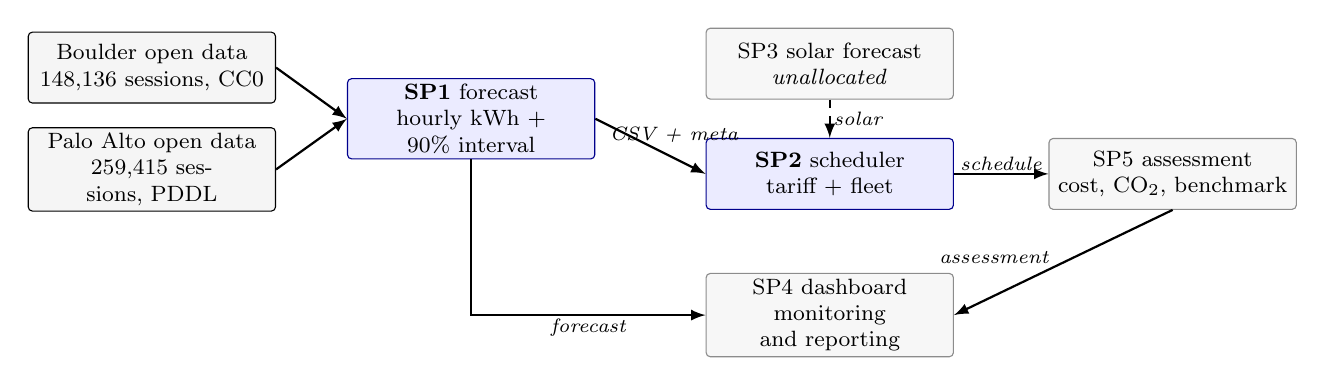
\begin{tikzpicture}[
  font=\footnotesize,
  box/.style={draw, rounded corners=1.5pt, align=center, minimum height=9mm,
              text width=30mm, inner sep=2pt, fill=white},
  data/.style={box, fill=black!4},
  own/.style={box, fill=blue!8, draw=blue!55!black},
  other/.style={box, fill=black!3, draw=black!45},
  ar/.style={-latex, thick},
  lab/.style={font=\scriptsize\itshape, inner sep=1pt}
]
\node[data] (b) {Boulder open data\\148{,}136 sessions, CC0};
\node[data, below=3mm of b] (p) {Palo Alto open data\\259{,}415 sessions, PDDL};
\node[own, right=9mm of b, yshift=-6.5mm] (sp1) {\textbf{SP1} forecast\\hourly kWh + 90\% interval};
\node[other, right=14mm of sp1, yshift=7mm] (sp3) {SP3 solar forecast\\\emph{unallocated}};
\node[own, right=14mm of sp1, yshift=-7mm] (sp2) {\textbf{SP2} scheduler\\tariff + fleet};
\node[other, right=12mm of sp2] (sp5) {SP5 assessment\\cost, CO$_2$, benchmark};
\node[other, below=8mm of sp2] (sp4) {SP4 dashboard\\monitoring and reporting};

\draw[ar] (b.east) -- (sp1.west);
\draw[ar] (p.east) -- (sp1.west);
\draw[ar] (sp1.east) -- node[lab, above, xshift=3mm]{CSV + meta} (sp2.west);
\draw[ar, dashed] (sp3.south) -- node[lab, right]{solar} (sp2.north);
\draw[ar] (sp2.east) -- node[lab, above]{schedule} (sp5.west);
\draw[ar] (sp5.south) -- node[lab, above left, pos=0.55]{assessment} (sp4.east);
\draw[ar] (sp1.south) |- node[lab, pos=0.75, below]{forecast} (sp4.west);
\end{tikzpicture}}
\captionof{figure}{Platform architecture. Blue boxes are the components this report builds; grey
boxes are the other sub-projects, shown only to fix the interfaces.}
\label{fig:arch}
\end{center}

\begin{zh}
图 1：平台架构。蓝色框是本报告构建的组件；灰色框是其他子项目，画出来只为固定接口——沿箭头流动的文件，其列定义由集成契约规定。SP3 目前未分配，按"缺省零光伏"处理。
\end{zh}

Electric vehicle (EV) adoption is adding load to distribution networks faster than network capacity
is being reinforced, and the timing of that load is set by drivers rather than by the network.
Uncoordinated charging concentrates demand in the hours when vehicles are parked and their owners
are available to plug in, which raises peak demand, raises the price paid for energy, and can force
curtailment of renewable generation that would otherwise have been absorbed. Coordinated charging
inverts the problem: the same energy can be delivered at a different time, so peak demand falls
without any reduction in the service provided. The platform in this project implements that
inversion as a software pipeline: forecast the demand, schedule it against a tariff and a
generation profile, display the result, and quantify what it saved.

\begin{zh}
电动汽车的普及正在给配电网加负荷，速度快于电网扩容；而这份负荷出现在什么时候，由车主决定，不由电网决定。无序充电把需求集中到"车停着、人方便插枪"的那几个小时，结果是抬高峰值、抬高用能价格，还可能逼得本可消纳的可再生发电被弃掉。有序充电把这个问题的方向反过来：同样的电量换个时间送出去，峰值就下降，而服务量一点没少。本项目把这个"反过来"做成一条软件流水线——预测需求、按电价与发电曲线排程、把结果显示出来、再核算省下了多少。
\end{zh}

The platform is split into five sub-projects with fixed interfaces. Sub-project 1 (SP1, this
report) converts charging session records into an hourly demand series and forecasts the next 24
hours with a prediction interval. SP2 schedules that demand against a time-of-use tariff and a
fleet of vehicles. SP3 supplies a solar generation forecast which SP2 may consume; it is not yet
allocated to a student, and the interface is defined so that its absence is treated as zero solar
rather than as a blocker. SP4 is the monitoring dashboard that consumes every other sub-project's
output file. SP5 assesses the economic and environmental outcome. Figure~\ref{fig:arch} shows the
data flow and the contract file carried on each edge.

\begin{zh}
平台拆成五个子项目，接口固定。子项目 1（SP1，即本报告）把充电会话记录转成小时级需求序列，并给出未来 24 小时的预测及其预测区间。SP2 依据分时电价与车队情况对该需求排程。SP3 提供光伏发电预测供 SP2 使用；它目前尚未分配给任何学生，接口按"缺省视为零光伏"设计，而不是当成阻塞项。SP4 是监控看板，消费其余各子项目的输出文件。SP5 评估经济与环境效果。图 1 给出数据流，以及每条箭头上承载的契约文件。
\end{zh}

The forecasting layer is the one that determines whether the rest of the platform can be evaluated
at all: a schedule is only as good as the demand it is built on, and a dispatch constraint has to
hold against the upper end of the forecast interval rather than against a point forecast. The
importance is measurable rather than rhetorical. On the primary site used in this report, if every
session charges as soon as it connects, the hourly peak reaches 362.5\,kWh against a forecast peak
of 94.5\,kWh, an amplification of 3.84, while total energy delivered moves by 0.05\,\%. The saving
available to the platform therefore lies in moving load in time, not in reducing it, and the size
of that saving is set by how well demand can be predicted and how tightly its uncertainty can be
bounded.

\begin{zh}
预测层决定的是"平台其余部分到底能不能被评估"：排程的质量上限，就是它脚下那份需求的质量；而调度约束必须对着预测区间的上界成立，不是对着点预测成立。这份重要性是可测的，不是修辞。在本报告的主站点上，如果每次充电一插枪就开始，小时峰值会达到 362.5 kWh，而预测峰值是 94.5 kWh，放大 3.84 倍，同时总送出电量只变动 0.05\%。所以平台能拿到的收益在于把负荷挪到别的时间，不在于少充电；而这个收益有多大，取决于需求能被预测到多准、不确定性又能被约束到多紧。
\end{zh}

% ---------------------------------------------------------------------------
\section{Literature Review}

\subsection{Forecasting EV charging demand}

Published work on station-level load forecasting divides into model-family comparisons and one
systematised review, and the model family that wins depends on the data rather than on the
architecture. Zhu et al.~\cite{Zhu2019ShortTermEVLoadDL} compare four deep architectures on hourly
station load and report a gated recurrent unit network as the best performer, framing the problem
as a large fleet power draw driven by stochastic driver behaviour.
Vishnu et al.~\cite{Vishnu2023ShortTermEVLoadTSMLDL} compare an auto-regressive model, support
vector regression and an LSTM on Adaptive Charging Network data, report the LSTM as best with
MAE 4\,kW and RMSE 5.9\,kW, and provide the most concrete published error figure in this strand.
Zhang et al.~\cite{Zhang2022MCCNNTCN} combine a multi-channel convolutional network with a temporal
convolutional network and add meteorological and calendar covariates, improving on an ANN by
14.09\,\%, on an LSTM by 25.13\,\% and on a TCN by 4.48\,\%. Ge et
al.~\cite{Ge2020SpatialTemporalEVLoadProfile} instead use a random forest with harmony-search
tuning and construct the spatial-temporal load of vehicle clusters bottom-up.
Alaraj et al.~\cite{Alaraj2025MLChargingDemandReview} survey the field and state the ordering that
this project adopts: unmanaged adoption risks network instability, smart charging mitigates it, and
smart charging presupposes an accurate forecast.

\begin{zh}
站点级负荷预测的既有工作大致分两类：模型族之间的比较，与一篇系统综述；而胜出的模型族取决于数据，不取决于架构。Zhu 等比较四种深度架构在小时级站点负荷上的表现，报告门控循环单元网络（GRU）最好，并把问题刻画为"由随机性驾驶行为驱动的大规模车队功率抽取"。Vishnu 等在 Adaptive Charging Network 数据上比较自回归模型、支持向量回归与 LSTM，报告 LSTM 最佳，MAE 4 kW、RMSE 5.9 kW，是这一支里最具体的已发表误差数字。Zhang 等把多通道卷积网络与时序卷积网络结合，并加入气象与日历协变量，相对 ANN 提升 14.09\%、相对 LSTM 25.13\%、相对 TCN 4.48\%。Ge 等换了另一条路：用和声搜索调参的改进随机森林，再自下而上构造车辆集群的时空负荷。Alaraj 等综述该领域，并道出本项目采纳的先后次序——大规模无管理接入带来电网不稳定风险，智能充电可以缓解，而智能充电以准确预测为前提。
\end{zh}

\begin{table}[H]
\centering
\caption{Representative forecasting studies and what they establish for this project.}
\label{tab:lit}
\small
\renewcommand{\arraystretch}{1.15}
\begin{tabular}{@{}p{3.3cm}p{3.6cm}p{3.0cm}p{5.0cm}@{}}
\toprule
Study & Data and level & Model & What it settles here \\
\midrule
Zhu et al.~\cite{Zhu2019ShortTermEVLoadDL} & Station, hourly & GRU & Recurrent models are competitive at station level \\
Vishnu et al.~\cite{Vishnu2023ShortTermEVLoadTSMLDL} & ACN, station & LSTM & MAE 4\,kW; a reference error figure from the same data family \\
Zhang et al.~\cite{Zhang2022MCCNNTCN} & Urban station, 15\,min & CNN + TCN & Calendar and weather covariates improve accuracy \\
Ge et al.~\cite{Ge2020SpatialTemporalEVLoadProfile} & Cluster & Random forest & Spatial aggregation needs a bottom-up construction \\
Alaraj et al.~\cite{Alaraj2025MLChargingDemandReview} & Review & --- & Forecast first, schedule second \\
\bottomrule
\end{tabular}
\end{table}

\begin{zh}
表 1：代表性预测研究与它们为本项目确立的结论。四列依次为：研究、数据与粒度、模型、在此确立的结论。
\end{zh}

\subsection{From session records to hourly load profiles}

The project's central data-engineering assumption is that a table of sessions, each carrying a
connection time, a disconnection time and a metered energy quantity, can be turned into an hourly
power profile. Yi and Scoffield~\cite{Yi2018ResidentialLoadProfileGeneration} estimate the
distribution of charging duration conditional on parking duration and generate synthetic behaviour
that preserves the parking-to-travel dependency. Uimonen and
Lehtonen~\cite{Uimonen2020OfficeBuildingOccupancy} derive office-building profiles from measured
charger occupancy, the closest published analogue to the workplace site used here.
Munkhammar et al.~\cite{Munkhammar2014BernoulliPEVCharging} reduce a Monte Carlo state-of-charge
simulation to hour-by-hour Bernoulli distributions of plug-in status and show that the aggregate
over many vehicles is approximately normal, which is the formal basis for turning per-vehicle
plug-in indicators into a fleet profile. Lahariya et
al.~\cite{Lahariya2020SyntheticDataGenerator} model arrivals as a Poisson-like process with
connection time dependent on arrival time, and von
Hoffen~\cite{vonHoffen2016ChargingTransactionAnalytics} makes the complementary point that
transaction records acquire analytical value only after enrichment with context. The consequence
for this project is that charging duration is modelled as a function of occupancy rather than as a
constant rate, which is why a session's metered energy is spread across its charging window in
proportion to overlap instead of being divided by a rated power.

\begin{zh}
本项目最核心的数据工程假设是：一张会话表——每次充电带连接时间、断开时间与计量电量——可以转成小时级功率曲线。Yi 与 Scoffield 以停车时长为条件估计充电时长的分布，并生成保留"停车—出行"依赖关系的合成行为。Uimonen 与 Lehtonen 从实测的充电桩占用率推导办公楼曲线，这是与本项目所用办公/市政站点最接近的已发表对应物。Munkhammar 等把蒙特卡洛的荷电状态仿真压缩成逐小时的"插枪状态"伯努利分布，并证明大量车辆聚合之后近似正态——这正是把逐车插枪指示量变成车队曲线的形式依据。Lahariya 等把到达建模为类泊松过程、让连接时长依赖到达时刻；von Hoffen 则补上另一点：交易记录只有经过上下文增补之后才具备分析价值。对本项目的推论是：充电时长应被视为占用率的函数，而不是一个常数速率——所以一次会话的计量电量是按重叠比例摊到它跨过的那些小时上的，而不是除以额定功率。
\end{zh}

\subsection{Tariffs, scheduling and peak reduction}

Chen et al.~\cite{Chen2012ValleyFilling} formulate joint optimal power flow and EV charging for a
fleet with heterogeneous charging-rate limits and characterise the optimal offline schedule as a
valley-filling profile, giving both a centralised and a decentralised online algorithm that tracks
it; this is the benchmark against which a scheduling heuristic can be judged approximately optimal.
Ramadan et al.~\cite{Ramadan2018PeakShavingValleyFilling} solve the related peak-shaving problem
with particle swarm optimisation and allow vehicle-to-grid discharge during peaks. On the tariff
side, Davis and Bradley~\cite{Davis2012TOURatesEfficacy} test whether time-of-use rates actually
shift charging and find that for plug-in hybrids the extra fuelling cost of charging off-peak can
cancel the incentive, so tariff response is not free and a cost-saving result that assumes it is
free overstates the benefit. Szinai et al.~\cite{Szinai2020ReducedGridOperatingCosts} link mobility
and dispatch models for California and report that 0.95--5 million managed vehicles avoid
USD 120--690 million in annual operating costs, up to 10\,\%, and cut renewable curtailment by up
to 40\,\%, while noting that overnight time-of-use charging increases curtailment at similar cost
savings. Dixon et al.~\cite{Dixon2020MinimiseEmissionsWindCurtailment} schedule against grid carbon
intensity and wind availability, reducing average charging emissions from 35--56 to
28--40\,gCO\textsubscript{2}/km. Cost and curtailment are therefore separately measurable
objectives that can move in opposite directions, and a schedule has to state which one it
optimises.

\begin{zh}
Chen 等把最优潮流与车队充电联合建模，针对充电速率上限异质的车队，把离线最优排程刻画为"填谷"曲线，并给出集中式与去中心化的在线算法去跟踪它；这是判断启发式排程"接近最优"的基准。Ramadan 等用粒子群算法求解相关的削峰填谷问题，并允许在峰值时段由车网反向放电。电价这一侧，Davis 与 Bradley 检验分时电价是否真的改变了充电行为，发现对插电混动车而言，避开高峰充电所多付的燃料成本可能抵消掉电价激励——所以电价响应不是免费的，一个假定它免费的节省结论会高估收益。Szinai 等把出行与调度模型连起来做加州算例，报告 95 万至 500 万辆受管车辆每年可省 1.2 亿至 6.9 亿美元运行成本（最高 10\%），并把可再生弃电削减最多 40\%；但同时指出，夜间的分时电价充电会在成本节省相近的情况下"增加"弃电。Dixon 等按电网碳强度与风电可用性排程，把平均充电排放从 35--56 gCO$_2$/km 降到 28--40~gCO$_2$/km。因此成本与弃电是两个可分别度量、且可能反向运动的目标，排程必须声明它优化的是哪一个。
\end{zh}

\subsection{Open data and measured grid impact}

Amara-Ouali et al.~\cite{AmaraOuali2021EVLoadOpenDataReview} survey open data for reproducible EV
load research, searching more than 860 repositories and returning roughly 60 datasets, and motivate
the survey by the field's shortage of charging-station data of realistic consistency. That finding
framed the dataset choice made here: official municipal releases were selected on provenance, a
public-domain or open licence, metered energy per session, and downloadable access without
registration. Li et al.~\cite{Li2025UrbanEV} publish UrbanEV, covering charging-space availability
and electricity consumption in Shenzhen at hourly resolution for more than 20{,}000 stations, and
Lee et al.~\cite{Lee2021ACNSim} present ACN-Sim, which also serves as the DOI-bearing citation for
the Adaptive Charging Network dataset. On the impact side, Powell et
al.~\cite{Powell2022ChargingInfrastructureGridImpacts} evaluate charging demand against a 2035
economic dispatch for the Western Interconnection and find peak net demand rising by up to
25\,\% under forecast adoption and 50\,\% in a full-electrification stress test, with the
counter-intuitive result that locally optimised charging combined with a high share of home
charging can strain the grid, while uncontrolled \emph{daytime} charging reduces storage, ramping
and emissions. Verma et al.~\cite{Verma2021ReviewImpactsDistributionNetwork} review
distribution-network impacts across penetration levels, supporting the treatment of impact as a
function of fleet size rather than as a fixed property of EVs.

\begin{zh}
Amara-Ouali 等为"可复现"的电动汽车负荷研究调查开放数据，检索 860 余个仓库、得到约 60 个数据集，并以"该领域缺少一致性可用的充电站数据"作为调查动机。这一发现框定了本项目的选数据标准：官方市政发布、公有领域或开放许可、逐会话计量电量、无需注册即可下载。Li 等发布 UrbanEV，覆盖深圳两万余个站点的车位可用性与用电量，小时级、六个月；Lee 等给出 ACN-Sim，它同时充当 Adaptive Charging Network 数据集的带 DOI 引用。影响这一侧，Powell 等把充电需求放进美国西部互联电网 2035 年的经济调度中评估，发现按预测渗透率峰值净需求上升最多 25\%、全面电气化压力测试下上升 50\%，并给出一个反直觉结论：局部优化充电叠加高比例家充，可能"加重"电网压力，而"无管理的白天充电"反而降低储能需求、爬坡与排放。Verma 等按渗透率水平综述配电网影响，支持"影响是车队规模的函数"而不是电动汽车的固定属性。
\end{zh}

\subsection{Significance and the gap addressed}

Three conclusions follow from the review and shape the specification. First, one-hour resolution
with a rolling-origin out-of-sample protocol and explicit naive baselines is the minimum design
under which a reported accuracy means anything; the reviewed papers mostly compare model families
against each other, and a learned model that does not beat persistence has demonstrated nothing.
Second, published absolute errors come from other datasets and larger sites, so they are context
rather than targets. Third, session-level open data with metered energy is scarce, and the Chinese
official route was closed after verification: the national charging platform publishes monthly
aggregates for members, not per-session records, so the forecasting work rests on two municipal
releases.

\begin{zh}
综述给出三条结论，并塑造了本报告的规格。第一，1 小时分辨率 + 滚动起点样本外协议 + 明确的朴素基线，是"报出来的精度能算数"的最低设计；被综述的论文大多只在模型族之间互比，而一个打不过持续法的学习模型并没有证明任何东西。第二，已发表的绝对误差来自别的数据集、更大的站点，只能当背景，不能当靶子。第三，带计量电量的会话级开放数据很稀缺，而中国官方路线经核实已关闭：全国充电平台对会员发布的是月度聚合，不是逐会话记录，所以预测工作落在两份市政发布上。
\end{zh}

What is missing in that literature, and what this project therefore specifies, is a forecasting
layer built on open municipal session data that (i) reports accuracy against naive baselines
rather than only against other learned models, (ii) carries a calibrated prediction interval that
is evaluated by its coverage rather than assumed, and (iii) demonstrates that the result transfers
to a second city without retuning. The next section turns the gap into objectives.

\begin{zh}
文献里缺的、因而本报告要规定的是：一个建立在开放市政会话数据上的预测层，它（i）对着朴素基线报精度，而不只对着别的学习模型；（ii）带一个经过校准、并以"覆盖率"而非假定来评价的预测区间；（iii）证明结果能在不重调的情况下迁移到第二个城市。下一节把这个缺口转成目标。
\end{zh}

% ---------------------------------------------------------------------------
\section{SMART Objectives}

Four objectives are specified. Each states a measurable target and the date by which it is met, and
each maps to a task in the work plan of Section~\ref{sec:plan}.

\begin{enumerate}[label=O\arabic*.]
  \item \textbf{A reproducible demand series from open session data.} By 30 October 2026, convert
        the two official municipal session datasets into gap-free hourly demand series in UTC, with
        a contract-validated CSV plus metadata sidecar and at least 50 automated tests covering
        ingestion, aggregation and time-zone handling. \emph{Achieved: 77 tests pass; both series
        are produced by one command from a checksummed download.}
  \item \textbf{Day-ahead forecasts that beat persistence on both sites.} By 31 January 2027,
        produce 1--24\,h forecasts that reduce WAPE against the naive same-hour-yesterday baseline
        by at least 15\,\% on the primary site and by at least 10\,\% on the validation site, with
        measured coverage of the nominal 90\,\% interval within $\pm$3 percentage points.
        \emph{Partially achieved: 19\,\% and 18\,\% reductions, coverage 91.0\,\% and 90.5\,\%.}
  \item \textbf{A quantified peak-shifting target for the scheduler.} By 30 April 2027, quantify,
        for the primary site, the peak reduction and cost difference between uncontrolled charging
        and a schedule built on the forecast, and deliver both series to SP5 for the assessment.
        \emph{In progress: the uncontrolled baseline is built; the scheduled series depends on SP2.}
  \item \textbf{An interface that other sub-projects consume unchanged.} By 30 April 2027, deliver
        the forecast as a contract file that SP2, SP4 and SP5 read without transformation, with the
        interval columns populated and the method recorded in the sidecar.
        \emph{Partially achieved: the contract file and sidecar exist and are versioned.}
\end{enumerate}

\begin{zh}
本报告规定四条目标；每条都给出可测目标值与达成日期，并对应 §6 工作计划中的一项任务。

\textbf{O1 可复现的需求序列}：到 2026 年 10 月 30 日，把两份官方市政会话数据转成 UTC 下无缺口的小时级需求序列，配一个通过契约校验的 CSV 与元数据旁文件，并有至少 50 个覆盖摄取、聚合与时区处理的自动化测试。已达成：77 个测试通过，两条序列由一条命令从带校验和的下载生成。

\textbf{O2 两站都跑赢持续法的日前预测}：到 2027 年 1 月 31 日，产出 1--24 小时预测，使 WAPE 相对"昨天同一小时"朴素基线在主站点至少降低 15\%、在验证站点至少降低 10\%，且标称 90\% 区间的实测覆盖率落在 $\pm$3 个百分点之内。部分达成：分别降 19\% 与 18\%，覆盖率 91.0\% 与 90.5\%。

\textbf{O3 给调度器的削峰量化目标}：到 2027 年 4 月 30 日，在主站点上量化"无序充电"与"基于预测的排程"之间的峰值差与成本差，并把两条序列交给 SP5 做评估。进行中：无序基线已建成，排程序列依赖 SP2。

\textbf{O4 其他子项目不改一行就能消费的接口}：到 2027 年 4 月 30 日，把预测交付为契约文件，SP2、SP4、SP5 无需转换即可读取，区间两列已填，方法记录在旁文件里。部分达成：契约文件与旁文件已存在并带版本。
\end{zh}

The key contributions are the use of official municipal session data as a forecasting basis where
the field mostly relies on proprietary or single-site records, a direct multi-horizon formulation in
which the forecast step is an input feature rather than a recursion, and an interval that is
evaluated by its coverage instead of being asserted.

\begin{zh}
主要贡献有三：在学界多依赖专有数据或单站点记录的地方，用官方市政会话数据作为预测基础；采用"把预测步长当作输入特征"的直接多步形式，取代递归；以及一个以覆盖率被评价、而不是只被声明的预测区间。
\end{zh}

% ---------------------------------------------------------------------------
\section{Technical Background}

\subsection{Hypothesis and method}

The hypothesis is that aggregate charging demand at a municipal or workplace site is governed by
calendar structure and by the recent level of demand, so that a gradient-boosted model on
target-hour calendar values plus forecast-origin lags, with the forecast horizon supplied as a
feature, predicts one to twenty-four hours ahead more accurately than persistence at every horizon.
Two consequences follow. Because the horizon is a feature, one model serves all horizons and needs
no recursion, which removes the error compounding that a one-step model accumulates when iterated.
Because every feature is either a calendar value of the \emph{target} interval or a lag anchored at
the \emph{origin}, no information from the future can enter the model; a regression test recomputes
each lag from the raw series and fails if any feature can see its own target.

\begin{zh}
假设是：市政或办公站点的聚合充电需求由日历结构与近期需求水平主导；于是在"目标小时的日历量 + 预测起点的滞后"上训练的梯度提升模型，把预测步长本身作为特征输入时，对 1 至 24 小时的每一个步长都比持续法更准。由此有两个推论。其一，因为步长是特征，一个模型服务所有步长、无需递归，从而消除了单步模型迭代所累积的误差放大。其二，因为每个特征要么是"目标"区间的日历量、要么是锚定在"起点"的滞后，未来信息无法进入模型；一个回归测试会从原始序列重算每个滞后，任何特征若能看到自己的目标就会失败。
\end{zh}

\subsection{Data and derivation}

Two official municipal releases are used. The City of Boulder, Colorado, publishes 148{,}136
charging transactions at 50 city-owned Level-2 stations between January 2018 and December 2023,
with metered energy per session, under CC0; it is the primary site and supplies 1.253\,GWh. The
City of Palo Alto, California, publishes 259{,}415 sessions at 47 stations between July 2011 and
January 2021 under the PDDL, supplying 2.216\,GWh; it is used only for validation. Both are
session-level records with connection time, disconnection time and metered energy, which is the
minimum schema the derivation needs.

\begin{zh}
使用两份官方市政发布。科罗拉多州博尔德市在 2018 年 1 月至 2023 年 12 月间、于 50 个市属二级充电站记录了 148,136 次充电交易，含逐会话计量电量，许可为 CC0；它是主站点，提供 1.253 GWh。加州帕洛阿尔托市在 2011 年 7 月至 2021 年 1 月间、于 47 个站点记录了 259,415 次会话，许可为 PDDL，提供 2.216 GWh；它只用于验证。两份都是逐会话记录，带连接时间、断开时间与计量电量——这正是派生所需的最小 schema。
\end{zh}

Each session's metered energy is spread over the hourly intervals it actually overlaps, in
proportion to the overlap, and the timeline is closed into a gap-free hourly grid. This is the
occupancy-conditional treatment argued for by~\cite{Yi2018ResidentialLoadProfileGeneration} and
\cite{Uimonen2020OfficeBuildingOccupancy}, with one limitation inherited from the source: the
records carry no within-session power taper, so a constant rate is assumed inside a session. The
assumption is recorded in the output metadata rather than left implicit.

\begin{zh}
每次会话的计量电量按重叠比例摊到它真正跨过的那些小时格上，时间轴补成无缺口的小时网格。这是 Yi 与 Scoffield、Uimonen 与 Lehtonen 所主张的"以占用率为条件"的处理，但继承了源数据的一处限制：记录里没有会话内部的功率衰减，因此会话内部按恒定速率假定。该假定写进输出的元数据，而不是留在暗处。
\end{zh}

\subsection{Evaluation and interval construction}

Seven models are scored: three naive baselines (same hour yesterday, same hour last week, and an
hour-of-week profile) and four learned models (ridge regression, random forest, gradient boosting
and XGBoost). Evaluation is a rolling-origin backtest in which every model is retrained at every
origin using only targets strictly before that origin, and each origin forecasts the following
24 hours; origins are anchored to local midnight, so each is a genuine day-ahead forecast. Accuracy
is reported as WAPE, the total absolute error divided by total demand, which stays stable when many
intervals carry near-zero demand, alongside MAE, RMSE and $R^2$. The interval is empirical:
$\hat{y} \pm 1.645\,\sigma$, where $\sigma$ is the residual standard deviation at the same horizon
in the backtest, clipped at zero because demand cannot be negative.

\begin{zh}
共评七个模型：三个朴素基线（昨天同一小时、上周同一小时、周内小时画像）与四个学习模型（岭回归、随机森林、梯度提升、XGBoost）。评估是滚动起点回测：每个起点上所有模型都用严格早于该起点的目标重新训练，每个起点预测其后 24 小时；起点锚定在本地午夜，因此每个都是真正的日前预测。精度以 WAPE 报告——总绝对误差除以总需求——它在许多小时格需求近零时依然稳定；同时报 MAE、RMSE 与 $R^2$。区间是经验式的：$\hat{y} \pm 1.645\sigma$，其中 $\sigma$ 是回测中同一步长的残差标准差，并在零处截断，因为需求不可能为负。
\end{zh}

\subsection{Preliminary results}

\begin{table}[H]
\centering
\caption{Rolling-origin results, targets strictly out of sample. Boulder: 25 origins, 600 hours.
Palo Alto: 14 origins, 336 hours. The interval is nominal 90\,\%.}
\label{tab:results}
\small
\renewcommand{\arraystretch}{1.15}
\begin{tabular}{@{}lrr@{}}
\toprule
Metric & Boulder (primary) & Palo Alto (validation) \\
\midrule
WAPE, gradient boosting & 0.292 & 0.549 \\
WAPE, naive same hour yesterday & 0.360 & 0.670 \\
Relative reduction in WAPE & 19\,\% & 18\,\% \\
MAE (kWh per hour) & 8.37 & 7.02 \\
RMSE (kWh per hour) & 11.39 & 9.70 \\
$R^2$ & 0.763 & 0.466 \\
Measured coverage of the 90\,\% interval & 91.0\,\% & 90.5\,\% \\
\bottomrule
\end{tabular}
\end{table}

\begin{zh}
表 2：滚动起点结果，目标严格处于样本外。博尔德 25 个起点、600 小时；帕洛阿尔托 14 个起点、336 小时；区间为标称 90\%。各行依次是：梯度提升的 WAPE、朴素"昨天同一小时"的 WAPE、WAPE 相对降幅、MAE、RMSE、$R^2$、90\% 区间的实测覆盖率。
\end{zh}

On the primary site the gradient-boosted model reaches a WAPE of 0.292 against 0.360 for the naive
daily baseline, a reduction of 19\,\%, with $R^2$ of 0.763 and a measured interval coverage of
91.0\,\% against a nominal 90\,\%; the mean interval width is 33.2\,kWh per hour. The same
pipeline, with no parameter changed, reaches 0.549 against 0.670 on the validation site, still a
reduction of 18\,\%, at 90.5\,\% coverage. The normalised error is higher on the validation site
while the absolute error per hour is comparable (7.02 against 8.37\,kWh), because the two windows
differ in scale and in period; the absolute figures are therefore not comparable across sites, and
the claim made here is the within-site relative gain, which repeats at 18\,\%. That repetition is
the evidence that the gain comes from the method rather than from tuning.
Figure~\ref{fig:fc} shows the last week of the evaluation window.

\begin{zh}
在主站点上，梯度提升模型取得 WAPE 0.292，相对朴素日基线 0.360 降低 19\%，$R^2$ 为 0.763，标称 90\% 区间的实测覆盖率为 91.0\%，区间平均宽度 33.2 kWh/小时。同一套管线不改任何参数，在验证站点上取得 0.549 对 0.670，仍是 18\% 的下降，覆盖率 90.5\%。验证站的归一化误差更高，而每小时的绝对误差相当（7.02 对 8.37 kWh），这是因为两个窗口在规模与时期上都不同；因此绝对数字不能跨站比较，本报告主张的是同站内的相对增益，而它在两站都复现为 18\% 左右。这种复现正是"增益来自方法而非调参"的证据。图 2 给出评估窗口的最后一周。
\end{zh}

\begin{figure}[tbp]
\centering
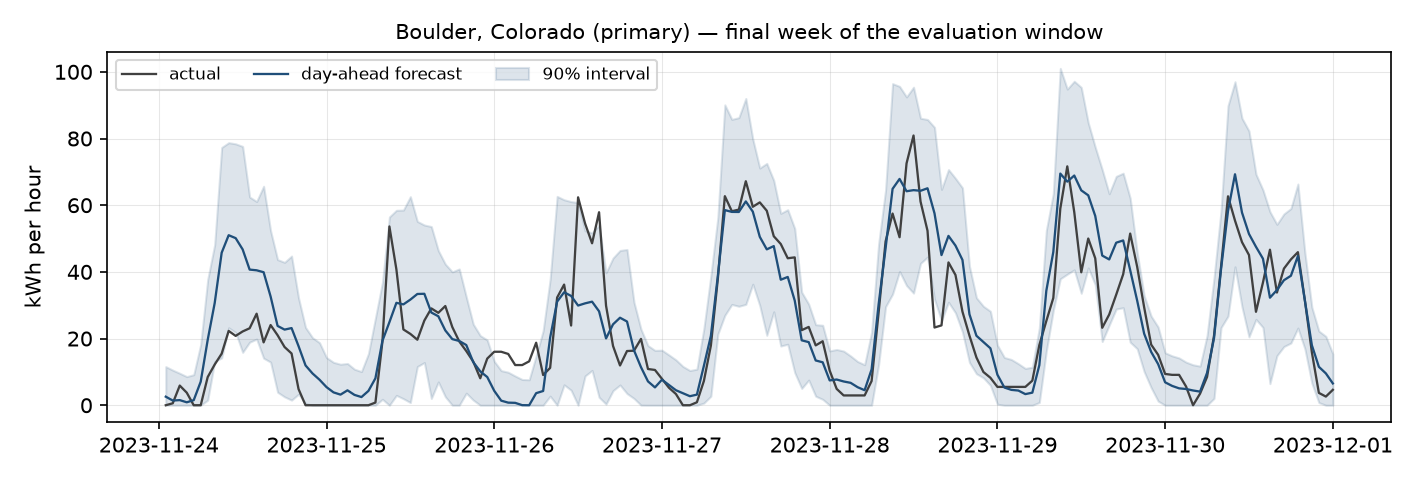
\includegraphics[width=0.94\textwidth]{../phase1-report/figures/sp1-forecast-vs-actual.png}
\caption{Metered demand, day-ahead forecast and the 90\,\% prediction interval over the final week
of the evaluation window on the primary site. The band widens where demand is volatile because it
is built from the residual quantiles of the backtest at each horizon.}
\label{fig:fc}
\end{figure}

\begin{zh}
图 2：主站点评估窗口最后一周的实测需求、日前预测与 90\% 预测区间。区间在需求波动处变宽，因为它是按每个步长的回测残差分位数构造的，不是拍一个固定百分比。
\end{zh}

Two properties of the data constrain the platform that consumes these forecasts. Both sites peak in
the middle of the working day, at 11:00 in Boulder and 12:00 in Palo Alto, and bottom out at 04:00
with a peak-to-trough ratio of about nineteen; there is no residential evening peak, because this
is public charging rather than home charging. A scheduler that assumes the evening peak of the
project brief would therefore optimise the wrong hours, which is a finding the Phase-3 design has
to carry.

\begin{zh}
数据有两处性质约束着消费这些预测的平台。两站都在工作日的中段见顶——博尔德 11:00、帕洛阿尔托 12:00——并在 04:00 落到谷底，峰谷比约十九倍；没有居民晚高峰，因为这是公共充电而不是家充。因此，一个沿用任务书里"晚高峰"假设的排程器会优化错的小时，这是 Phase 3 设计必须承接的发现。
\end{zh}

% ---------------------------------------------------------------------------
\section{References}

\begin{zh}
参考文献不译：作者、题名、期刊与 DOI 保留原文，便于检索与核对。本报告的 20 条引用与文献综述共用同一批经 Crossref 逐条解析验证的条目。
\end{zh}

\bibliographystyle{IEEEtran}
\bibliography{../literature-review/references}

% ---------------------------------------------------------------------------
\clearpage
\section{Measurable Outcomes and Work Plan}\label{sec:plan}

\begin{table}[H]
\centering
\caption{Main tasks, measurable targets and dates. Type: S = software, D = data, A = analysis,
T = theoretical.}
\label{tab:plan}
\small
\renewcommand{\arraystretch}{1.12}
\begin{tabular}{@{}p{0.6cm}p{6.6cm}p{6.0cm}p{2.1cm}@{}}
\toprule
Type & Task & Measurable target & Due \\
\midrule
D & Acquire and register official session datasets & Two series reproducible from a checksummed download & Sep 2026 \\
S & Session-to-hourly pipeline with contract IO & Gap-free hourly CSV plus metadata, $\geq$50 tests & Oct 2026 \\
S & Feature set, direct multi-horizon models, backtest & WAPE reported against three naive baselines & Oct 2026 \\
A & Interval construction and coverage check & Measured coverage within $\pm$3\,pp of nominal & Nov 2026 \\
A & Cross-site validation without retuning & Relative WAPE reduction $\geq$10\,\% on site 2 & Nov 2026 \\
S & Tariff-aware features and interface freeze & Contract v2 consumed by SP2 without change & Dec 2026 \\
A & Interim report and presentation & Submitted 8 Jan; presented 11--22 Jan & Jan 2027 \\
A & Phase-3 evaluation with SP2 and SP5 & Peak, cost and CO$_2$ deltas quantified & Apr 2027 \\
T & Dissertation and poster & Submitted 30 Apr; poster 19--21 Apr & Apr 2027 \\
\bottomrule
\end{tabular}
\end{table}

\begin{zh}
表 3：主要任务、可测目标与日期。类型一列：S = 软件、D = 数据、A = 分析、T = 理论。九行的顺序就是执行顺序，最后一列是截止月份；其中"11 月做区间校准、12 月冻结接口"两行是这份计划里最容易被拖延的两个节点。
\end{zh}

\begin{figure}[H]
\centering
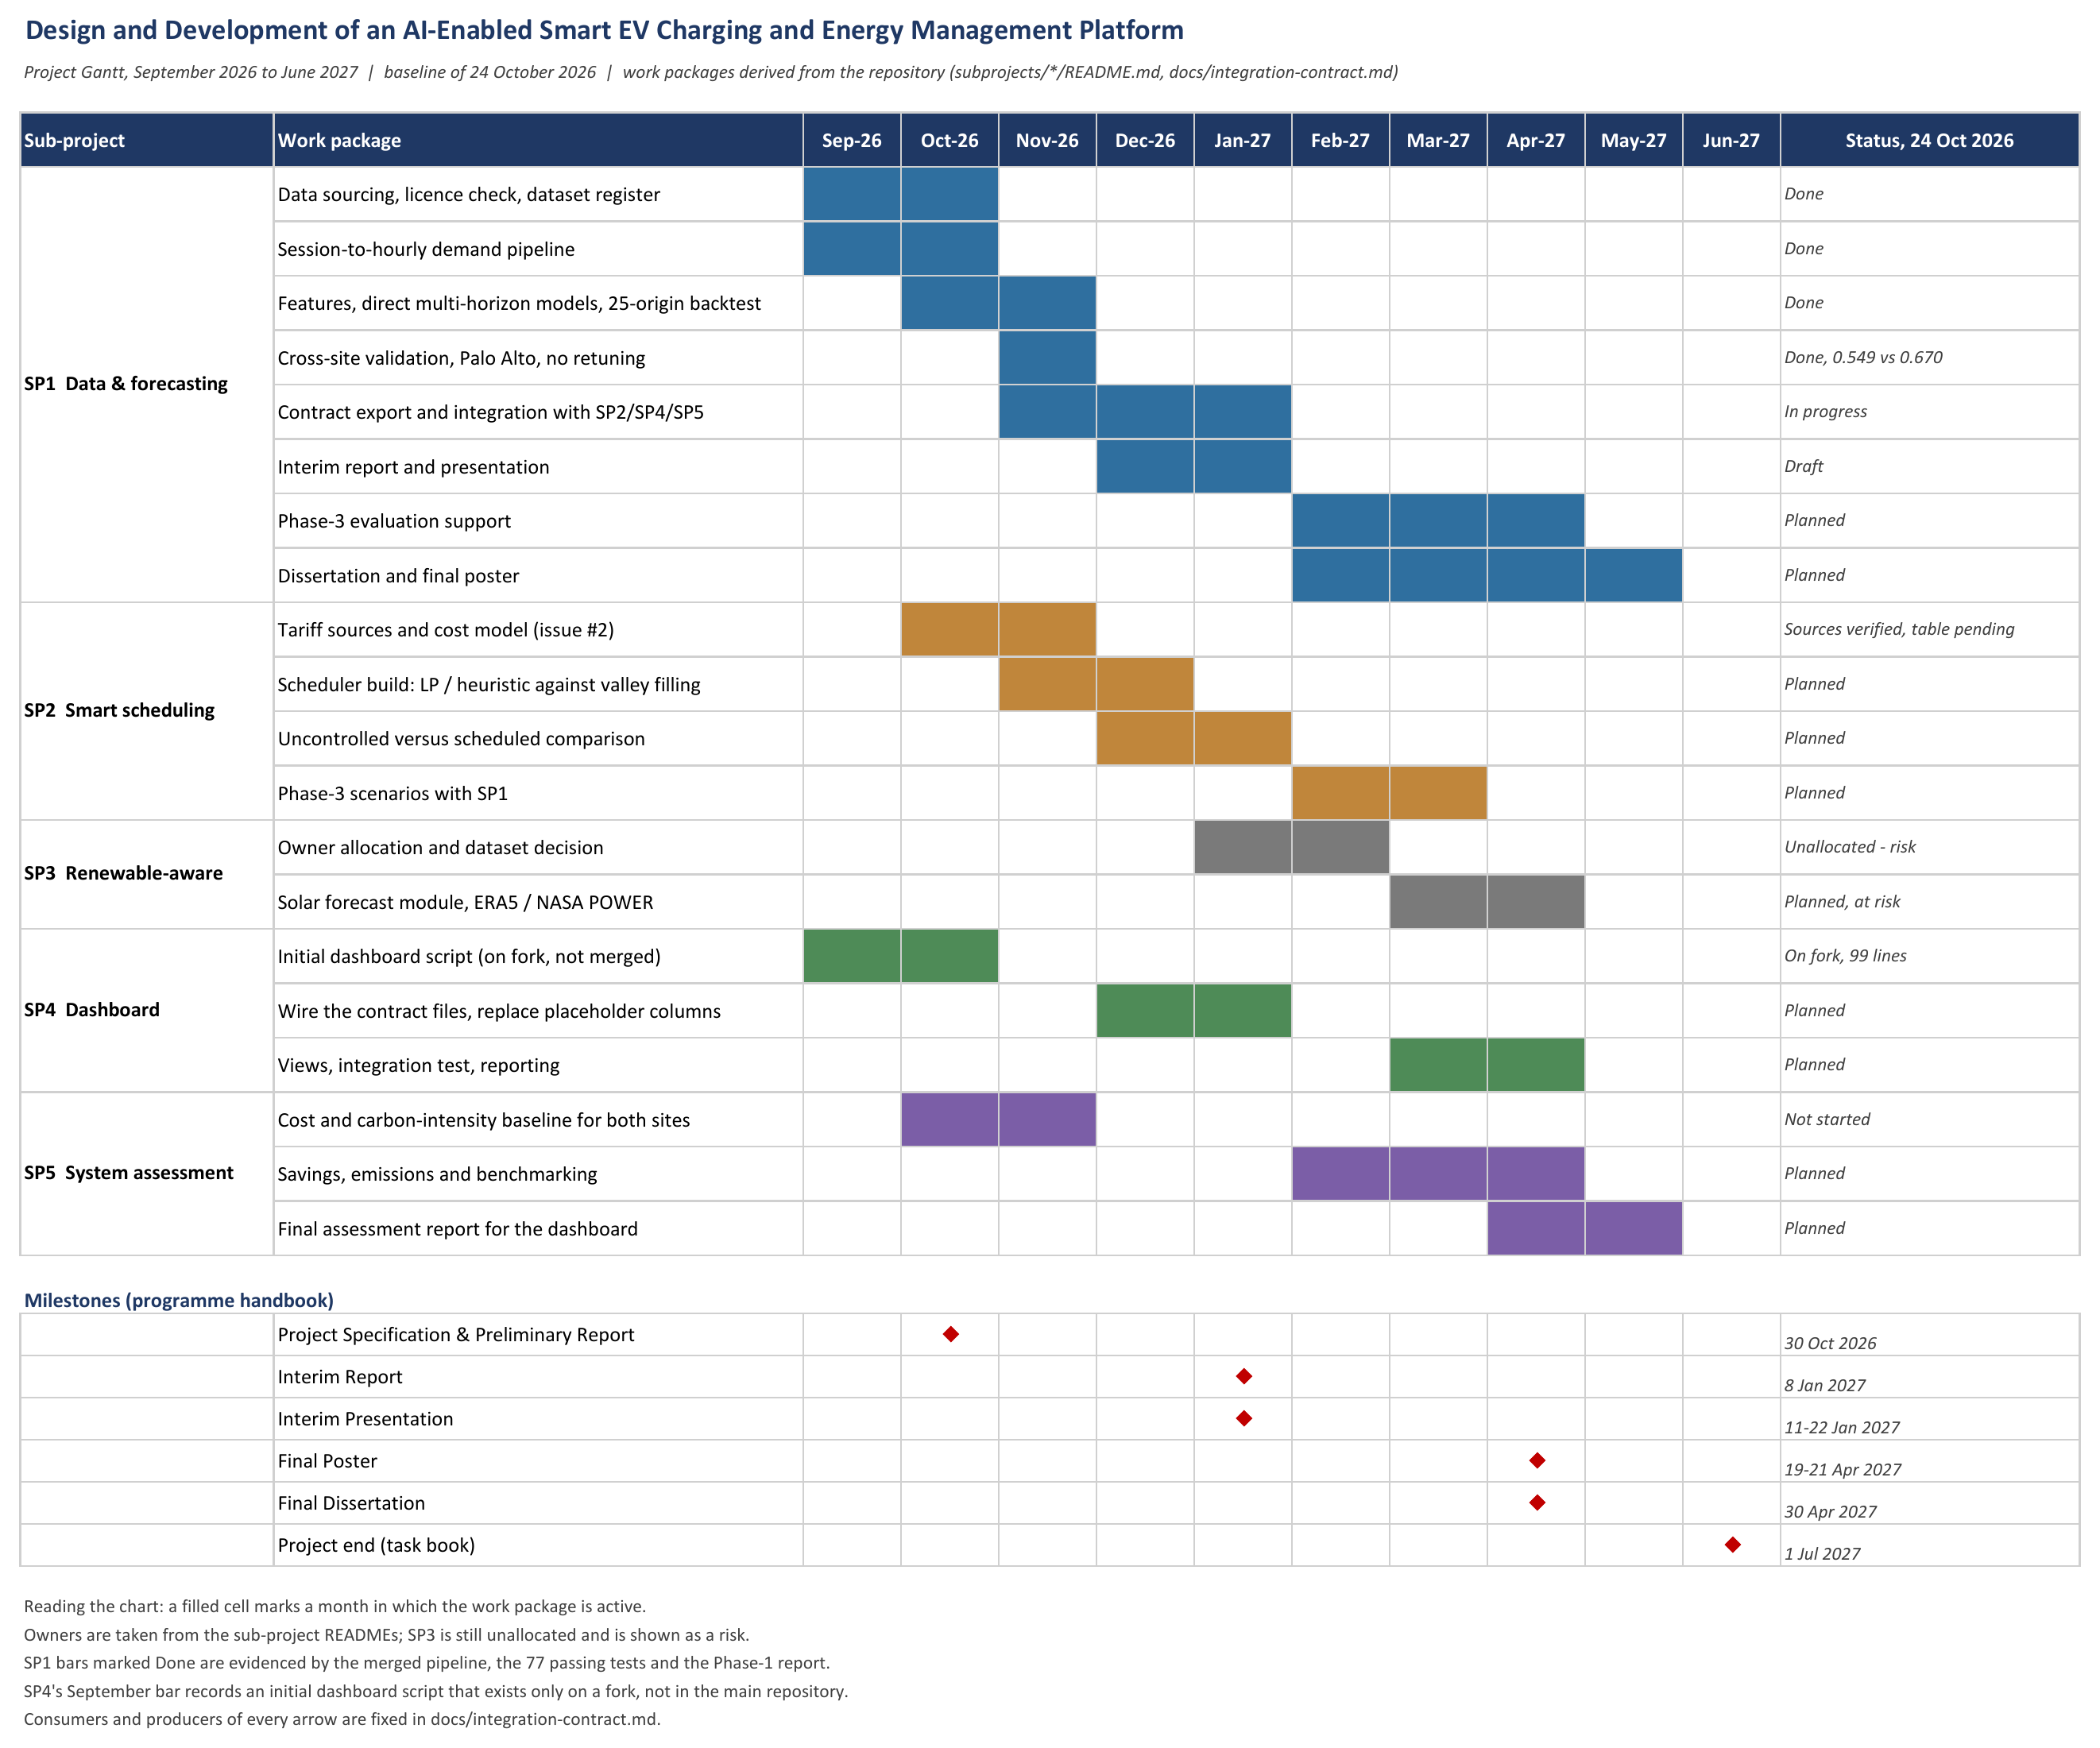
\includegraphics[width=0.86\textwidth]{plan/gantt.png}
\caption{Work plan for this sub-project, September 2026 to June 2027: the five main tasks of the
task book broken into sub-tasks, the other sub-projects shown only as external dependencies, and
milestone dates taken from the FYP handbook. Month spans are planning judgements. The workbook
\code{gantt.xlsx} carries this sheet plus a whole-platform view for group planning.}
\label{fig:gantt}
\end{figure}

\begin{zh}
图 3：本子项目的工作计划，2026 年 9 月至 2027 年 6 月。任务书五条主线拆成子任务；其他子项目只以"外部依赖"（灰底）出现，不在这里替别人排期；里程碑日期取自 FYP 手册。为什么只画自己的活：手册 p12 要求甘特图是"导师已指定的主线之下的子任务"，p13 又规定协作项目中由导师分配"各自独立的工作包、各有自己的目标"。月份跨度是排期判断（仓库不记录月份），只有最右列状态是 2026-10-24 的事实。工作簿 \code{gantt.xlsx} 含本表，另有一张供小组讨论用的全平台视图。
\end{zh}

\end{document}
